\chapter{Dynamic Model} \label{ch:model}

***************************************\\
%INTRO 

The dynamics of the QR-Load system are described by the laws of kinematics and the application of Newton's laws or Lagrangian mechanics. Opposed to the classical modeling techniques, it is also possible to describe the system's configuration space as a differentiable manifold with the tools of differential geometry. \\

In order to simulate the system and the effects of Geometric Control, the system is modeled with the following assumptions.\\

In order to avoid complexities and ambiguities associated with attitude representations such as \textit{Euler-Angles} or \textit{quaternions}, the attitude dynamics of the Quadrotor-Load system can be globally expressed on the Special Orthogonal Group $SO(3)$
***************************************\\

The derived mathematical model is represented by a set of dynamic equations commonly used for rigid body transformations. Considering the properties of the system, the QR is modeled as a rigid body. The motion of a rigid body can be described by a translation of the center of mass and a rotation about the center of mass. This principle describes a rigid body with six degrees of freedom, driven by forces and moments. \\

\section{Modeling Assumptions} 
The Quadrotor model representation is shown in Figure \ref{fig:mod.model}. Three Cartesian coordinate frames are defined:\v{5}
\begin{itemize}
	\setlength\itemsep{.2pt}
	\item The body-fixed reference frame \lsymb{$ \{\mathcal{B}\} $}{Body Frame} (Body Frame)
	%								\nomenclature{$ \{\mathcal{B}\} $}{Body Frame}
	\subitem with unit vectors \lsymb{$ \{\mathbf{b}_1,\mathbf{b}_2,\mathbf{b}_3\} $}{Unit vectors along the axes of $ \{\mathcal{B}\} $} along the axes
	\item The ground-fixed reference frame \lsymb{$ \{\mathcal{I} \}$}{Inertial World Frame} (Inertial Frame)
	%								\nomenclature{$ \{\mathcal{I} \}$}{Inertial World Frame}
	\subitem with unit vectors \lsymb{$ \{\mathbf{e}_1,\mathbf{e}_2,\mathbf{e}_3\} $}{Unit vectors along the axes of $ \{\mathcal{I}\} $} along the axes								
	\item The intermediary frame \lsymb{$ \{\mathcal{C} \}$}{Intermediary Frame}, ($ \{\mathcal{I} \}$ rotated by the yaw angle $ \psi $) 
	%								\nomenclature{$ \{\mathcal{C} \}$}{Intermediary Frame}
	\subitem with unit vectors \lsymb{$ \{\mathbf{c}_1,\mathbf{c}_2,\mathbf{c}_3\} $}{Unit vectors along the axes of $ \{\mathcal{C}\} $} along the axes								
\end{itemize}

\begin{figure}[h!]
	\centering
	\makebox[\textwidth][c]{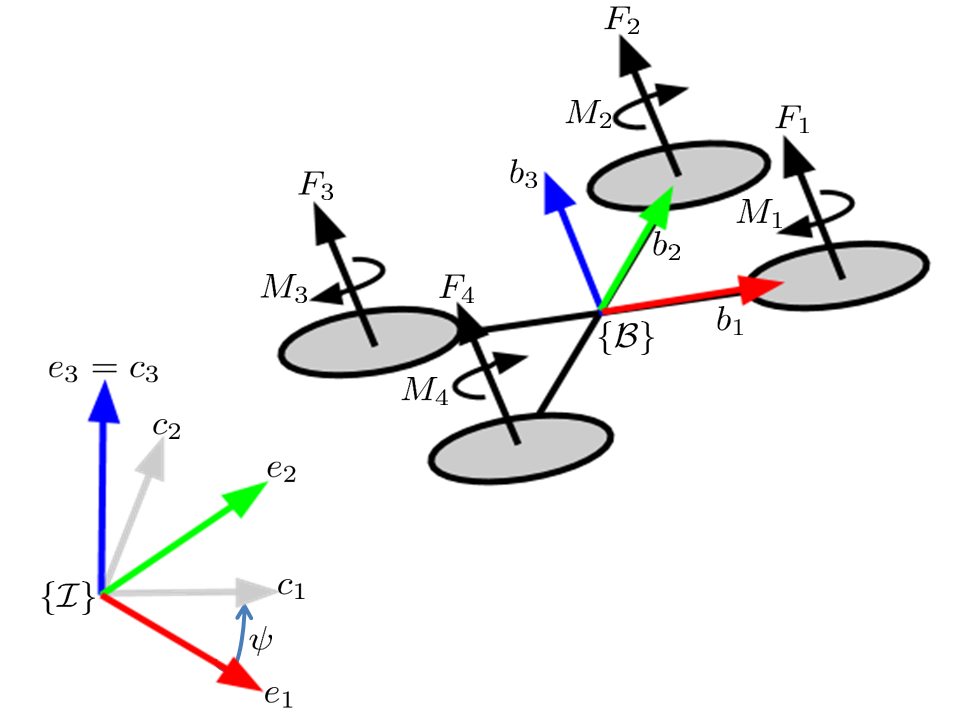
\includegraphics[width=.5\paperwidth]{./StyleStuff/qrmodelppt.png}}
	\caption{Quadrotor model representation\label{fig:mod.model}}
\end{figure}	

\begin{figure}[h!]
	\centering
	\makebox[\textwidth][c]{\includegraphics[width=.5\paperwidth]{./StyleStuff/dcsc.png}}
	\caption{Quadrotor with Load model representation\label{fig:mod.modelQRL}}
\end{figure}	

The position of the body frame is described by a vector evolving on $ \mathbb{R}^3 $, and is represented with respect to the inertial frame. The orientation of the body frame with respect to the inertial frame evolves on a nonlinear space, for which several methods exist to describe this, such as \textit{Euler Angles}, quaternions or rotation matrices. 

Table \ref{tab:mod.assumptions} shows the most common assumptions that are used for modeling the QR, simplifying the complexity of the model.

\begin{table}[h!]
	\centering
	\begin{tabular}{|p{\textwidth}|}
		\hline
		\tabitem The rotation of the Earth does not affect the flight of the QR\\
		\tabitem The structure of the QR is rigid and symmetric. \\
		\hspace{4mm} Elastic deformations and shock (sudden accelerations) of the QR are ignored.\\										
		\tabitem The mass distribution of the QR is symmetrical in the x-y plane.\\
		\tabitem The inertia matrix is time-invariant.\\
		\tabitem Aerodynamic effects acting on the QR are neglected.\\
%		\hspace{4mm} An indoor environment guarantees the absence of unpredictable disturbances like wind\\ 
%		\hspace{4mm} gusts. The model complexity decreases without modeling the effects of wind.\\ 	
		\tabitem The propellers are rigid $ \Rightarrow $ The thrust produced by rotor $ i $ is parallel to the axis of rotor $ i $.\\
		\tabitem The air density around the QR is constant.\\
		\tabitem Drag factor \lsymb{$ d $ }{Drag factor} and thrust factor \lsymb{$ b $}{Thrust factor} are constant.\\
		\hspace{4mm} Thrust force $ F_i $ and drag moment \lsymb{$ \tau_{drag,i} $}{Drag moment generated by each propellor} of each propeller is proportional to the square of \\
		\hspace{4mm} the propeller speed. $ F_i = b\omega_i^2$ and $ \tau_{drag,i} = d\omega_i^2$, where \lsymb{$ \omega_i $}{Angular velocity of rotor $ i $ around its axis, $ i=\{1,2,3,4\} $} is the rotor speed.\\
		\hline
	\end{tabular}
	\caption{Modeling assumptions Quadrotor model}
	\label{tab:mod.assumptions}
\end{table}

\begin{table}[h!]
	\centering
	\begin{tabular}{|p{\textwidth}|}
		\hline
		\tabitem The cable is modeled as a rigid and massless cable. \\
		\tabitem The tension in the cable is considered to be non-zero.\\
		\hspace{4mm} This implies that the subsystem consisting of a Quadrotor and Load in free fall is disregarded.\\		 
		\tabitem Aerodynamic effects acting on the load are neglected.
		\tabitem Assumption \\
		\hspace{4mm} Details Assumption 2\\
		\hline
	\end{tabular}
	\caption{Modeling assumptions Quadrotor+Load model}
	\label{tab:mod.assumptionsQRL}
\end{table}



***************************************\\
\cite{Goodarzi2013a} includes uncertainties in the translational dynamics and rotational dynamics. Out of the scope, might be interesting.\\
***************************************\\


***************************************\\
\begin{figure}[h!]
	\centering
	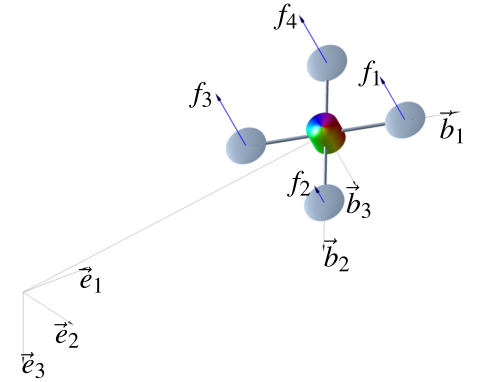
\includegraphics[width=.45\textwidth]{./StyleStuff/LeeQRmodel.png}
	\caption{\label{fig:}}
\end{figure}		
***************************************\\


\section{Geometric Modeling}\label{sec:mod.geometric}

%HOE DAN? 
Differential Geometry is used to analyze the underlying geometric properties of a system.

With geometric modeling the configuration space is a group manifold instead of a Euclidean space. The kinetic and potential energies are expressed in terms of this configuration space and its velocities.

***************************************\\
Rigid Body Attitude Dynamics:
\begin{align}\label{eq:eomrigidbody}
J\dot{\Omega}+\Omega\times J\Omega &= mg\rho\times R^Te_3+u\\
\dot{R} &= R\hat{\Omega}
\end{align}
***************************************\\


***************************************\\
\cite{Lee}
Why is this used, pros/cons\\

%		\subsection{Lagrangian System}
Mechanics studies the dynamics of physical bodies acting under forces and potential fields. 
In Lagrangian mechanics, the trajectories are obtained by finding the paths that minimize the integral of a Lagrangian over time, called the action integral. 
Rigid body dynamics are characterized by Lagrangian/Hamiltonian dynamics. The dynamics of a Lagrangian system has unique geometric properties and these are exploited to obtain Euler-Lagrange equations. The resulting intrinsic form of the Euler-Lagrange equations are more compact than equations expressed in terms of local coordinates.

When angular errors are large, the difference in Euler angles is no longer a good metric to define the orientation error. Local coordinates often require symbolic computational tools due to complexity of multi-body systems. Hence, the error is rather written as the required 3-D rotation to get from the current to the desired orientation. As a result, the equations of motion and the control systems can be developed on a configuration manifold in a coordinate-free, compact, unambiguous manner, while singularities of local parameterization are avoided to generate agile maneuvers in a uniform way. 				

Most of nonlinear dynamics and control problems are studied in a linear space.\\
\begin{equation}\label{key}
\dot{x}=f(t,x,u), \quad x\in\mathbb{R}^n, u\in\mathbb{R}^m, f:\mathbb{R}^{n+m+1}\rightarrow\mathbb{R}^n
\end{equation}

Geometric Mechanics and Control is used to understand the structure of the equations of motion of a system in order to facilitate its analysis and design. The evolution of the system and the design of controllers is done on a nonlinear manifold.\\

In mathematics there are different types of singularity, in these cases we are talking about the situation where:\\
Many points in one representation are mapped onto a single point in another representation.\\
Infinitesimal changes close to the singularity in one representation may cause large changes in the other representation.

Computational Geometric Mechanics and Control\\
Computation algorithms must be developed which preserve the geometric properties of a mechanical system.\\
Robust and careful numerical implementation of geometric control theory to complex engineering systems.\\
Provides nontrivial maneuvers that are globally valid on a nonlinear configuration manifold.

Assumptions\\

Problems, singularities with Euler-Angles\\
Other attitude representations, such as exponential coordinates, quaternions, or Euler
angles, can also be used following standard descriptions, but each of the representations has a disadvantage
of introducing an ambiguity or singularity.
Why charts on $ SO(3) $ \url{https://en.wikipedia.org/wiki/Charts_on_SO(3)}\\

\begin{equation}\label{key}
SO(3) \triangleq \left\lbrace R\in\mathbb{R}^{3\times3}:RR^T=I_{3\times3},det(R)=1\right\rbrace 
\end{equation}

Rotational matrices with determinant 1 is a Lie group: $ SO(3) $\\
$ SO(3) $ is the group of all rotations about origin of three-dimensional Euclidean space\\
Rotation about the origin is a transformation that preserves the origin, Euclidean distance and orientation.\\
Every rotation has a unique inverse rotation and the identity map satisfies the definition of a rotation.\\
Possible ways to represent rotations: orthogonal matrices with determinant 1, axis and rotation angle, geometric algebra as a rotor, sequence of three rotations about three fixed axes; Euler Angles\\
Lie group is a group that is also a differentiable manifold.\\
Differentiable manifold is a type of manifold that is locally similar enough to a linear space to allow to do calculus.\\
Manifold is a topological space that locally resembles Euclidean space near each point. Each point of an n-dimensional manifold has a neighbourhood that is homeomorphic to the n-dimensional Euclidean space.\\
Homeomorphism is a continuous function between topological spaces that has a continuous inverse function. (mug transforms to a torus)\\


Difference $ SO(3) $ and $ so(3) $ >> $ SO(3) $ is a Lie Group, $ so(3) $ is Lie Algebra\\
Special Orthogonal group
\begin{equation}\label{key}
SO(3)=\left\lbrace R\in\mathbb{R}^{3\times3}|R^TR=I,\quad detR=1\right\rbrace 
\end{equation}
The group operation for $ SO(3) $ corresponds to matrix multiplication.\\
The attitude kinematics equation is given by
\begin{equation}\label{key}
\dot{R}=R\hat{\Omega}
\end{equation}
where $ \Omega\in\mathbb{R}^3 $ is the angular velocity represented in the body fixed frame. The hat map $ \hat{\cdot}:\mathbb{R}^3\rightarrow \mathfrak{so}(3)$ is an isomorphism between $ \mathbb{R}^3 $ and the set of $ 3\times 3 $ skew symmetric matrices. The Lie algebra $ \mathfrak{so}(3) $ is defined by
\begin{equation}\label{key}
\hat{\Omega}=\begin{bmatrix}
0&-\Omega_3&\Omega_2\\
\Omega_3&0&-\Omega_1\\
-\Omega_2&\Omega_1&0
\end{bmatrix}
\end{equation}

Rotation formalisms in three dimensions \url{https://en.wikipedia.org/wiki/Rotation_formalisms_in_three_dimensions#cite_note-5}\\
Combining two successive rotations, each represented by an Euler axis and angle, is not straightforward, and in fact does not satisfy the law of vector addition, which shows that finite rotations are not really vectors at all. It is best to employ the rotation matrix or quaternion notation, calculate the product, and then convert back to Euler axis and angle.

Euler Angles\\
However, the definition of Euler angles is not unique and in the literature many different conventions are used. These conventions depend on the axes about which the rotations are carried out, and their sequence (since rotations are not commutative). Therefore, Euler angles are never expressed in terms of the external frame, or in terms of the co-moving rotated body frame, but in a mixture. Other conventions (e.g., rotation matrix or quaternions) are used to avoid this problem.

***************************************\\
Geometric mechanics is a modern description of classical mechanics from the perspective of differential geometry \cite{Bullo2005,Jurdjevic1997}. It explores the geometric structure of a Lagrangian or Hamiltonian system through the concept of vector fields, symplectic geometry, and symmetry techniques. Geometric mechanics provides fundamental insights into mechanics and yields useful tools for dynamics and control theory.

In control systems engineering, the underlying geometric features of a dynamic system are often not considered carefully. For example, many control systems are developed for the standard form of ordinary differential equations, namely $ \dot{x}=f(x,u) $, where the state and the control input are denoted by $ x $ and $ u $. It is assumed that the state and the control input lie in Euclidean spaces, and the system equations are defined in terms of smooth functions between Euclidean spaces. However, for many interesting mechanical systems, the configuration space cannot be expressed globally as a Euclidean space.

In \cite{Lee2008} dynamics and optimal control problems for rigid bodies are studied, incorporating their geometric features. The focus lies on obtaining geometric properties of the dynamics of rigid bodies, how their configuration can be described and how these geometric properties are utilized in control system analysis and design. Computational methods for rigid bodies, that preserve the underlying Lagrangian/Hamiltonian system structure of rigid body dynamics as well as the Lie group structure of the configurations are developed.

\subsection{Lie Group Configuration Manifold} 
The configuration of a rigid body can be described by the location of its mass center and the orientation of the rigid body in a 3-D space. The location of the rigid body can be expressed in Euclidean space, but the attitude evolves in a nonlinear space that has a certain geometry. The attitude of a rigid body is defined as the direction of a body-fixed frame with respect to a reference frame, considered as a linear transformation on the vector space $ \mathbb{R}^3 $.\\
The attitude can be represented mathematically by a $ 3\times 3 $ orthonormal matrix. The set of $ 3\times3 $ orthonormal matrices with positive determinant is a manifold as it is locally diffeomorphic to a Euclidean space, and it also has a group structure with the group action of matrix multiplication. A smooth manifold with a group structure is referred to as a Lie group; the Lie group of $ 3\times 3 $ orthonormal matrices with positive determinant is referred to as the special orthogonal group, $ SO(3) $ \cite{Murray1994}.

The configuration manifold for the attitude dynamics of a rigid body is $ SO(3) $, and the configuration manifold for combined translational and rotational motion of a rigid body is the special Euclidean group $ SE(3) $, which is a semi-direct product of $ SO(3)  $ and $ \mathbb{R}^3 $. A direct product of the Lie groups $ SE(3), SO(3), \text{and } \mathbb{R}^n $ can represent the configuration of multiple rigid bodies, and it is also a Lie group since a product of Lie groups is also a Lie group. Therefore, the configuration manifold of an interconnection of rigid bodies is also a Lie group.


\subsection{QR-Load Modeling}	


\subsection{QR Modeling}	

***************************************\\
System Identification\\
Model Validation?\\

Pendulum $ \in S^2 $: Based on \cite{Lee2011}.
***************************************\\

\section{Classical Modeling}
 When assuming small angle maneuvers, \textit{Euler-angles} can be used to locally parameterize the orientation of the body-fixed reference coordinate frame with respect to the inertial reference coordinate frame. 

***************************************\\
A commonly used method for modeling a system is via Newton's law and Lagrangian mechanics. 
Based on Euler-Lagrange? $ \rightarrow $ Geometric Mechanics\\

Pro/Cons of Classical Modeling Techniques vs Geometric Modeling\\

Linearized model/State Space model vs. Geometric modeling\\
***************************************\\
		\subsection{QR Modeling}
		\subsection{QR-Load Modeling}	
		
		
		***************************************\\
\begin{equation}
		ax = 
		\begin{bmatrix}
					(f*m*sin(\phi_q)*sin(\psi_q) + f*m_l*sin(\phi_q)*sin(\psi_q) - f*m_l*cos(\theta)^2*sin(\phi_q)*sin(\psi_q) + f*m*cos(\phi_q)*cos(\psi_q)*sin(\theta_q) + f*m_l*cos(\phi_q)*cos(\psi_q)*sin(\theta_q) + l*m*m_l*v_\theta^2*cos(\theta)*sin(\phi) + f*m_l*cos(\phi)^2*cos(\theta)^2*sin(\phi_q)*sin(\psi_q) + l*m*m_l*v_\phi^2*cos(\theta)^3*sin(\phi) - f*m_l*cos(\phi_q)*cos(\psi_q)*cos(\theta)^2*sin(\theta_q) + f*m_l*cos(\phi)^2*cos(\phi_q)*cos(\psi_q)*cos(\theta)^2*sin(\theta_q) + f*m_l*cos(\psi_q)*cos(\theta)*sin(\phi)*sin(\phi_q)*sin(\theta) + f*m_l*cos(\phi)*cos(\phi_q)*cos(\theta_q)*cos(\theta)^2*sin(\phi) - f*m_l*cos(\phi_q)*cos(\theta)*sin(\phi)*sin(\psi_q)*sin(\theta_q)*sin(\theta))/(m*(m + m_l))\\
			(l*m*m_l*v_\theta^2*sin(\theta) - f*m_l*cos(\psi_q)*cos(\theta)^2*sin(\phi_q) - f*m*cos(\psi_q)*sin(\phi_q) + f*m*cos(\phi_q)*sin(\psi_q)*sin(\theta_q) + f*m_l*cos(\phi_q)*cos(\theta)^2*sin(\psi_q)*sin(\theta_q) + l*m*m_l*v_\phi^2*cos(\theta)^2*sin(\theta) + f*m_l*cos(\phi)*cos(\phi_q)*cos(\theta_q)*cos(\theta)*sin(\theta) - f*m_l*cos(\theta)*sin(\phi)*sin(\phi_q)*sin(\psi_q)*sin(\theta) - f*m_l*cos(\phi_q)*cos(\psi_q)*cos(\theta)*sin(\phi)*sin(\theta_q)*sin(\theta))/(m*(m + m_l))\\
			-(g*m^2 + g*m*m_l - f*m*cos(\phi_q)*cos(\theta_q) - f*m_l*cos(\phi_q)*cos(\theta_q) + l*m*m_l*v_\theta^2*cos(\phi)*cos(\theta) + f*m_l*cos(\phi)^2*cos(\phi_q)*cos(\theta_q)*cos(\theta)^2 + l*m*m_l*v_\phi^2*cos(\phi)*cos(\theta)^3 + f*m_l*cos(\phi)*cos(\psi_q)*cos(\theta)*sin(\phi_q)*sin(\theta) - f*m_l*cos(\phi)*cos(\theta)^2*sin(\phi)*sin(\phi_q)*sin(\psi_q) - f*m_l*cos(\phi)*cos(\phi_q)*cos(\theta)*sin(\psi_q)*sin(\theta_q)*sin(\theta) - f*m_l*cos(\phi)*cos(\phi_q)*cos(\psi_q)*cos(\theta)^2*sin(\phi)*sin(\theta_q))/(m*(m + m_l))\\
			(- l*m*cos(\theta)*sin(\theta)*v_\phi^2 + f*cos(\psi_q)*cos(\theta)*sin(\phi_q) - f*cos(\phi)*cos(\phi_q)*cos(\theta_q)*sin(\theta) - f*cos(\phi_q)*cos(\theta)*sin(\psi_q)*sin(\theta_q) + f*sin(\phi)*sin(\phi_q)*sin(\psi_q)*sin(\theta) + f*cos(\phi_q)*cos(\psi_q)*sin(\phi)*sin(\theta_q)*sin(\theta))/(l*m)\\
			-(f*cos(\phi_q)*cos(\theta_q)*sin(\phi) + f*cos(\phi)*sin(\phi_q)*sin(\psi_q) - 2*l*m*v_\phi*v_\theta*sin(\theta) + f*cos(\phi)*cos(\phi_q)*cos(\psi_q)*sin(\theta_q))/(l*m*cos(theta))
		\end{bmatrix}
\end{equation}

		
		
		***************************************\\	
		
\section{Conclusion}

***************************************\\
Geometric Mechanics/Lie Groups/Lie Algebra is used in order to represent the dynamics of the system onto the nonlinear configuration manifold $ SE(3) $\\
Advantage of this method is\\
Enables to model on \\
That type of control is discussed in the next chapter


***************************************\\